\section{Begrenzerschaltung}
\subsection{Experimentelle Durchf\"uhrung}
Es wird die Schaltung wie in Abbildung 18 dargestellt mit einem Steckbrett aufgebaut. Zun\"achst wird das Verh\"altnis der Ein-/Ausgangsspannung mit der XY-Funktion des Oszilloskop bestimmt. Anschlie\ss end wird eine Diode durch eine Z-Diode ersetzt und wiederum das Verh\"altnis Ein-/Ausgangsspannung mit dem Oszilloskop dargestellt. 

\begin{figure}[ht]
\begin{center}
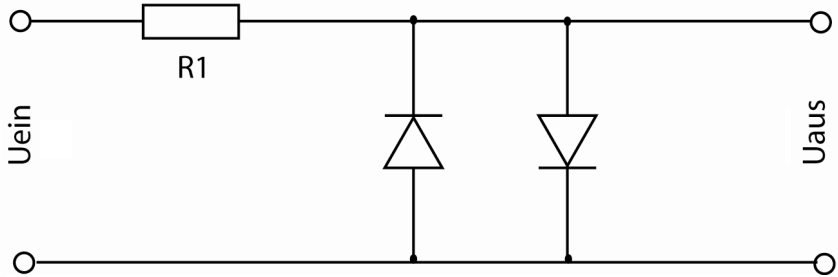
\includegraphics[scale=0.4]{schaltungVersuch4}
\caption{Begrenzerschaltung}
\end{center}
\end{figure} 
\noindent
Als n\"achstes wird die Begrenzerschaltung aus Abbildung 11 auf dem Steckbrett nachgebaut. Es wird wieder mithilfe der XY-Funktion des Oszilloskop die Spannung am Knoten K gegen die Spannung am Eingang dargestellt. Danach wird eine sinusf\"ormige Wechselspannung an den Eingang gelegt und die Messungen notiert. 
Dazu werden zwei \textbf{Si-Dioden} Typ:\textbf{1N4148} sowie einen Widerstand R$_1$ $=$ 1~$\Omega$ verwendet.
\begin{figure}[ht]
\begin{center}
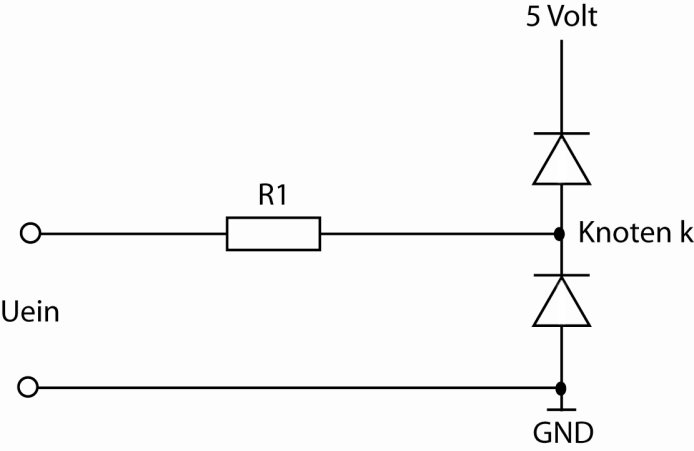
\includegraphics[scale=0.4]{schaltungVersuch4Version2}
\caption{Unbekannte Schaltung}
\end{center}
\end{figure}
\newpage
\subsection{Ergebnisse und Diskussion}
In der Abbildung 20 ist der Verlauf der Ausgangsspannung \"uber die Eingangsspannung dargestellt. Dabei ist zu beobachten, dass der Graph symmetrisch ist, da zwei gleiche \textbf{Si-Dioden} verwendet werden. Solang die Eingangsspannung die Schwellenspannung der \textbf{Si-Diode} nicht \"uberschreitet zeigt der Graph ein lineares Verhalten Ein-~/Ausgangsspannug d.h die Ausgangsspannung entspricht die Eingangsspannung. Falls die Eingangsspannung  die Schwellensapnnung \"uberchreitet, werden beide Diode leiten und die Ausgangsspannung wird auf ca. 0.7~$V$ limitiert.
\begin{figure}[!ht]
\begin{center}
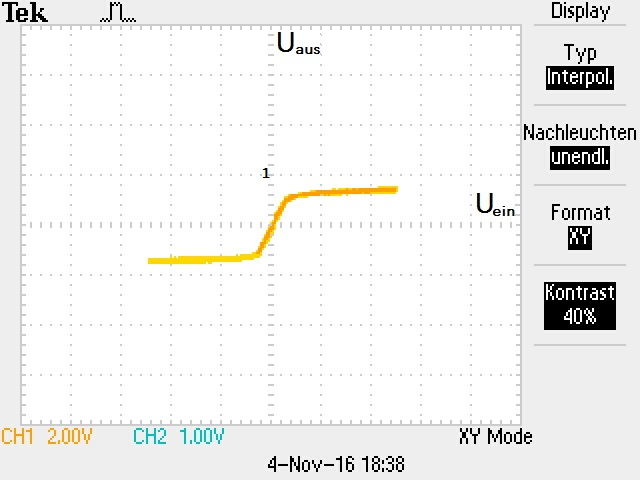
\includegraphics[scale=0.8]{Versuch4/TEK0003}
\caption{Begrenzerschaltung}
\end{center}
\end{figure}

\begin{figure}[!h]
In der Abbildung 21 ist der Verlauf der Ausgangsspannung \"uber der Eingangspannung dargestellt, dabei ist zu sehen, dass der Graph nach dem Tausch der \textbf{Si-Diode} mit einer \textbf{Z-Diode} nicht mehr symmetrisch ist. Dabei ist klar zu erkennen, dass in dem Graph nicht die Schwellenspannung zu sehen ist, sondern die Durchbruchsspannung der \textbf{Z-diode}, die bei einer Spannung von ca. 2.4~$V$ liegt. Die Schwellenspannung der \textbf{Si-Diode} ist die Gleiche, wie bei der \textbf{Z-Diode}.
(Da wir am Ende des Praktikums Probleme mit dem Speichern der Bilder hatten, wurde dieses Bild nach Einstellen des Funktionsgenerators auf (-5, 10~$V$) gemacht).
\begin{center}
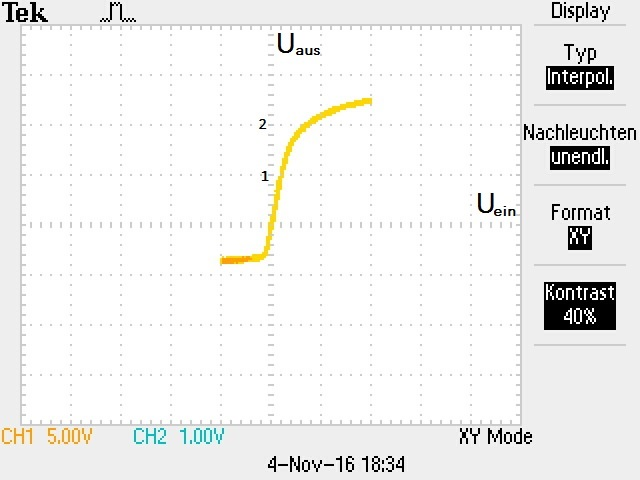
\includegraphics[scale=0.8]{Versuch4/TEK0001}
\caption{Begrenzerschaltung mit einer \textbf{Z-Diode}}
\end{center}
\end{figure}
\begin{figure}[!h]
Die Abbildung 22 stellt den Graph der unbekannten Schaltung aus Abbildung 12 dar. Zu erkennen ist, dass die Spannungsquelle von 5~$V$ die Schwellenspannung der Diode auf 5.7~$V$ hebt.
\begin{center}
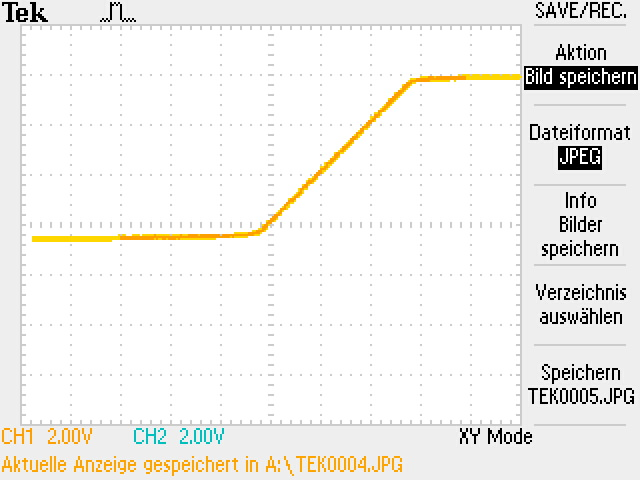
\includegraphics[scale=0.8]{Bilder/Versuch2/Limiter2}
\caption{Begrenzerschaltung 2}
\end{center}
\end{figure}